% !TeX TXS-program:compile = txs:///lualatex/[--shell-escape]

%----------------------- Преамбула -----------------------
\documentclass[ut8x, 14pt, oneside, a4paper]{extarticle}

\usepackage{extsizes} % Для добавления в параметры класса документа 14pt

% Для работы с несколькими языками и шрифтом Times New Roman по-умолчанию
\usepackage[english,russian]{babel}
\usepackage{fontspec}
\setmainfont{Times New Roman}
\usepackage[left=30mm,right=10mm,top=20mm,bottom=20mm]{geometry}
\usepackage{misccorr}
\usepackage{indentfirst}
\usepackage{enumitem}
\usepackage{pdfpages}
%\usepackage{ragged2e}
\setlength{\parindent}{1.25cm}
%\setlength{\parskip}{1em} % поменять
%\linespread{1.3}
\renewcommand{\baselinestretch}{1.5}
\setlist{nolistsep} % Отсутствие отступов между элементами \enumerate и \itemize

% Дополнительное окружения для подписей
\usepackage{array}
\newenvironment{signstabular}[1][1]{
	\renewcommand*{\arraystretch}{#1}
	\tabular
}{
	\endtabular
}

% Переопределение стандартных \section, \subsection, \subsubsection по ГОСТу;
% Переопределение их отступов до и после для 1.5 интервала во всем документе
\usepackage{titlesec}

\titleformat{\section}[block]
{\bfseries\normalsize\filcenter}{\thesection}{1em}{}

\titleformat{\subsection}[hang]
{\bfseries\normalsize}{\thesubsection}{1em}{}
\titlespacing\subsection{\parindent}{\parskip}{\parskip}

\titleformat{\subsubsection}[hang]
{\bfseries\normalsize}{\thesubsubsection}{1em}{}
\titlespacing\subsubsection{\parindent}{\parskip}{\parskip}

\newcommand{\specsection}[1]{\section*{#1}\addcontentsline{toc}{section}{#1}}

% Работа с изображениями и таблицами; переопределение названий по ГОСТу
\usepackage{caption}
\captionsetup[figure]{name={Рисунок},labelsep=endash}
\captionsetup[table]{singlelinecheck=false, labelsep=endash}

\usepackage{graphicx}
\usepackage{diagbox} % Диагональное разделение первой ячейки в таблицах

% Цвета для гиперссылок и листингов
\usepackage{color}

% Гиперссылки \toc с кликабельностью
\usepackage[linktoc=all]{hyperref}
\hypersetup{hidelinks}

% Листинги
%\setsansfont{Arial}
%\setmonofont{Courier New}

\usepackage{color} % Цвета для гиперссылок и листингов
%\definecolor{comment}{rgb}{0,0.5,0}
%\definecolor{plain}{rgb}{0.2,0.2,0.2}
%\definecolor{string}{rgb}{0.91,0.45,0.32}
%\hypersetup{citecolor=blue}
\hypersetup{citecolor=black}

\usepackage{listings}
\lstset{
	basicstyle=\footnotesize\ttfamily,
	language=XML, % Или другой ваш язык -- см. документацию пакета
	commentstyle=\color{comment},
	numbers=left,
	numberstyle=\tiny,
	numbersep=5pt,
	tabsize=4,
	extendedchars=\true,
	breaklines=true,
	keywordstyle=\color{blue},
	frame=b,
	stringstyle=\ttfamily\color{string}\ttfamily,
	showspaces=false,
	showtabs=false,
	xleftmargin=17pt,
	framexleftmargin=17pt,
	framexrightmargin=5pt,
	framexbottommargin=4pt,
	showstringspaces=false,
	inputencoding=utf8x,
	keepspaces=true
}

\DeclareCaptionLabelSeparator{line}{\ --\ }
\DeclareCaptionFont{white}{\color{white}}
\DeclareCaptionFormat{listing}{\colorbox[cmyk]{0.43,0.35,0.35,0.01}{\parbox{\textwidth}{\hspace{15pt}#1#2#3}}}
\captionsetup[lstlisting]{
	format=listing,
	labelfont=white,
	textfont=white,
	singlelinecheck=false,
	margin=0pt,
	font={bf,footnotesize},
	labelsep=line
}

\usepackage{ulem} % Нормальное нижнее подчеркивание
\usepackage{hhline} % Двойная горизонтальная линия в таблицах
\usepackage[figure,table]{totalcount} % Подсчет изображений, таблиц
\usepackage{rotating} % Поворот изображения вместе с названием
\usepackage{lastpage} % Для подсчета числа страниц

\makeatletter
\renewcommand\@biblabel[1]{#1.}
\makeatother

\usepackage{color}
\usepackage[cache=false, newfloat]{minted}
\newenvironment{code}{\captionsetup{type=listing}}{}
\SetupFloatingEnvironment{listing}{name=Листинг}

\usepackage{amsmath}
\usepackage{slashbox}


\begin{document}

\linespread{1.25}

\begin{titlepage}
	\noindent\begin{minipage}{0.05\textwidth}
		
\includegraphics[scale=0.3]{inc/bmstu.png}
	\end{minipage}
	\hfill
	\begin{minipage}{0.85\textwidth}\raggedleft
		\begin{center}
			\fontsize{12pt}{0.3\baselineskip}\selectfont \textbf{Министерство науки и высшего образования Российской Федерации \\ Федеральное государственное бюджетное образовательное учреждение \\ высшего образования \\ <<Московский государственный технический университет \\ имени Н.Э. Баумана \\ (национальный исследовательский университет)>> \\ (МГТУ им. Н.Э. Баумана)}
		\end{center}
	\end{minipage}
	\vspace*{-0.3cm}
	\begin{center}
		\fontsize{12pt}{0.1\baselineskip}\selectfont
		\noindent\makebox[\linewidth]{\rule{\textwidth}{1pt}} \makebox[\linewidth]{\rule{\textwidth}{4pt}}
	\end{center}
	\vspace*{-1.5cm}
	\begin{flushleft}
		\fontsize{12pt}{\baselineskip}\selectfont 
		
		ФАКУЛЬТЕТ ИУ <<Информатика и системы управления>>

		КАФЕДРА ИУ-7 <<Программное обеспечение ЭВМ и информационные технологии>>
	\end{flushleft}

	\vfill

	\begin{center}
		\fontsize{20pt}{\baselineskip}\selectfont

		\textbf{РАСЧЕТНО-ПОЯСНИТЕЛЬНАЯ ЗАПИСКА}

		\textbf{\textit{К НАУЧНО-ИССЛЕДОВАТЕЛЬСКОЙ РАБОТЕ}}

		\textbf{\textit{НА ТЕМУ:}}
	\end{center}

	\begin{center}
		\fontsize{20pt}{0.6cm}\selectfont 
		
		\textit{\bfseries{<<Применение сетей Петри для моделирования цифрового документооборота>>}}
		
	\end{center}

	\vfill
	
	\fontsize{12pt}{0.6cm}\selectfont
	Студент \hspace{1.1cm} ИУ7-75Б \hspace{3.83cm} \uline{\mbox{\hspace*{3.5cm}}}~ \textbf{Богаченко А. Е.}
	
	\vfill
	
	Руководитель НИР \hspace{4.8cm} \uline{\mbox{\hspace*{3.5cm}}}~ \textbf{Строганов Ю. В.}
	
	~~
	
	\textit{Рекомендуемая руководителем НИР оценка}~\uline{\mbox{\hspace*{3.5cm}}}
	
	\vfill

	\begin{center}
		\normalsize \textit{\the \year~г.}
	\end{center}
\end{titlepage}
\pagenumbering{gobble}
%\setlength\parindent{0pt}
\begin{center}
	\fontsize{12pt}{0.3\baselineskip}\selectfont \textbf{Министерство науки и высшего образования Российской Федерации \\ Федеральное государственное бюджетное образовательное учреждение \\ высшего образования \\ <<Московский государственный технический университет имени Н.Э. Баумана \\ (национальный исследовательский университет)>> \\ (МГТУ им. Н.Э. Баумана)}
\end{center}
\vspace*{-0.5cm}
\begin{center}
	\fontsize{12pt}{0.1\baselineskip}\selectfont
	\noindent\makebox[\linewidth]{\rule{\textwidth}{1pt}} \makebox[\linewidth]{\rule{\textwidth}{4pt}}
\end{center}

\begin{flushright}
	\fontsize{12pt}{0.4cm}\selectfont
	УТВЕРЖДАЮ\mbox{\hspace{2.5cm}}
	
	Заведующий кафедрой ИУ-7
	
	\uline{\mbox{\hspace{3cm}}} И. В. Рудаков
	
	<<16>> сентября 2023г.
\end{flushright}

\begin{center}
	\fontsize{20pt}{14pt}\selectfont

	\textbf{З А Д А Н И Е}
	
	\textbf{на выполнение научно-исследовательской работы}
\end{center}


\fontsize{12pt}{0.6cm}\selectfont	

по теме 
	
\makebox[\linewidth]{\textbf{<<Применение сетей Петри для моделирования цифрового документооборота>>}}
	
Студент группы \textbf{ИУ7-75Б}
	
\makebox[\linewidth]{\textbf{Богаченко Артём Евгеньевич}}
	
Направленность НИР
	
\makebox[\linewidth]{\textbf{учебная}}
	
Источник тематики
	
\makebox[\linewidth]{\textbf{НИР кафедры}}
	
График выполнения НИР: ~25\% к 6 нед., 50\% к 9 нед., 75\% к 12 нед., 100\% к 15 нед.
	
~~
	
\textit{\bfseries{Техническое задание}}

\textit{Провести обзор существующих методов моделирования цифрового документооборота. Провести анализ возможности применения сетей Петри для моделирования цифрового документооборота.}
	
~~
	
\textit{\bfseries{Оформление научно-исследовательской работы:}}

Расчетно-пояснительная записка на \textbf{12-20} листах формата А4.

\textit{\bfseries{Перечень графического (иллюстративного) материала:}}	

Презентация на \textbf{6-10} слайдах.

Дата выдачи задания <<16>> сентября 2023 г.	

~~

\textbf{Руководитель НИР} \hspace{3.6cm} \uline{\mbox{\hspace*{3.5cm}}} \hspace{1.1cm} \textbf{Строганов Ю. В.}

\hfill (Подпись, дата) \hspace{1.9cm} (Фамилия И. О) \hspace{1.2cm}

\textbf{Студент} \hspace{5.7cm} \uline{\mbox{\hspace*{3.5cm}}} \hspace{1.1cm} \textbf{Богаченко А. Е.}

\hfill (Подпись, дата) \hspace{1.9cm} (Фамилия И. О) \hspace{1.2cm}
	
\setlength{\parindent}{1.25cm}
%\setlength\parindent{0pt}
\begin{center}
	\fontsize{12pt}{0.3\baselineskip}\selectfont \textbf{Министерство науки и высшего образования Российской Федерации \\ Федеральное государственное бюджетное образовательное учреждение \\ высшего образования \\ <<Московский государственный технический университет имени Н.Э. Баумана \\ (национальный исследовательский университет)>> \\ (МГТУ им. Н.Э. Баумана)}
\end{center}
\vspace*{-0.5cm}
\begin{center}
	\fontsize{12pt}{0.1\baselineskip}\selectfont
	\noindent\makebox[\linewidth]{\rule{\textwidth}{1pt}} \makebox[\linewidth]{\rule{\textwidth}{4pt}}
\end{center}

\begin{flushright}
	\fontsize{12pt}{0.4cm}\selectfont
	УТВЕРЖДАЮ\mbox{\hspace{2.5cm}}
	
	Заведующий кафедрой ИУ-7
	
	\uline{\mbox{\hspace{3cm}}} И. В. Рудаков
	
	<<16>> сентября 2023г.
\end{flushright}

\begin{center}
	\fontsize{20pt}{14pt}\selectfont

	\textbf{З А Д А Н И Е}
	
	\textbf{на выполнение научно-исследовательской работы}
\end{center}


\fontsize{12pt}{0.6cm}\selectfont	

по теме 
	
\makebox[\linewidth]{\textbf{<<Применение сетей Петри для моделирования цифрового документооборота>>}}
	
Студент группы \textbf{ИУ7-75Б}
	
\makebox[\linewidth]{\textbf{Богаченко Артём Евгеньевич}}
	
Направленность НИР
	
\makebox[\linewidth]{\textbf{учебная}}
	
Источник тематики
	
\makebox[\linewidth]{\textbf{НИР кафедры}}
	
График выполнения НИР: ~25\% к 6 нед., 50\% к 9 нед., 75\% к 12 нед., 100\% к 15 нед.
	
~~
	
\textit{\bfseries{Техническое задание}}

\textit{Провести обзор существующих методов моделирования цифрового документооборота. Провести анализ возможности применения сетей Петри для моделирования цифрового документооборота.}
	
~~
	
\textit{\bfseries{Оформление научно-исследовательской работы:}}

Расчетно-пояснительная записка на \textbf{12-20} листах формата А4.

\textit{\bfseries{Перечень графического (иллюстративного) материала:}}	

Презентация на \textbf{6-10} слайдах.

Дата выдачи задания <<16>> сентября 2023 г.	

~~

\textbf{Руководитель НИР} \hspace{3.6cm} \uline{\mbox{\hspace*{3.5cm}}} \hspace{1.1cm} \textbf{Строганов Ю. В.}

\hfill (Подпись, дата) \hspace{1.9cm} (Фамилия И. О) \hspace{1.2cm}

\textbf{Студент} \hspace{5.7cm} \uline{\mbox{\hspace*{3.5cm}}} \hspace{1.1cm} \textbf{Богаченко А. Е.}

\hfill (Подпись, дата) \hspace{1.9cm} (Фамилия И. О) \hspace{1.2cm}
	
\setlength{\parindent}{1.25cm}

\normalsize

\pagenumbering{arabic}
\setcounter{page}{2}

\section*{РЕФЕРАТ}

Расчетно-пояснительная записка \pageref{LastPage} с., \totalfigures\ рис., \totaltables\ табл., 21 ист.

В работе представлен анализ применения стохастических временных сетей Петри для моделирования процессов цифрового документооборота.

Рассмотрены существующие системы цифрового документооборота. Рассмотрена классификация сетей Петри, составлена и проанализирована модель процесса утверждения темы для выпускной квалификационной работы. Составлен вывод на основе полученных результатов.

КЛЮЧЕВЫЕ СЛОВА

\textit{сети Петри, цифровой документоборот}

\pagebreak

\tableofcontents\normalsize


\pagebreak

\specsection{ВВЕДЕНИЕ}

Развитие области электронного документооборота (ЭДО) является одной из приоритетных и актуальных задач цифровизации государственных и частных секторов, об этом свидетельствует ежегодно увеличивающийся на 15\% объём электронного документооборота\cite{roseu}. 

Системы электронного документооборота (СЭД) должны отвечать высоким стандартам в области безопасности, эффективности и надёжности, где критическим показателем является своевременное исполнение процессов\cite{software-standards}. В связи с этим основное внимание в области ЭДО уделяется контролю процессов управления, нежели управлению потоком данных\cite{data-flow}. Система СЭД должна регулярно проходить проверки на соответствие стандартам и требованиям проектирования соответствующих систем\cite{gost}.

Цель работы -- провести обзор существующих решений в области СЭД и исследовать возможность применения сетей Петри для моделирования и формализации процессов ЭДО с целью разработки эффективных, безопасных и надёжных систем.

Для достижения этой цели требуется решить следующие задачи НИР:
\begin{enumerate}
	\item провести обзор существующих решений в области СЭД;
	\item исследовать возможность применения сетей Петри для моделирования ЭДО.
\end{enumerate}

\clearpage

\section{Анализ предметной области}
\subsection{Базовые понятия}

В данном разделе будет проведён анализ предметной области в контексте Российской Федерации и страна Организации Договора о коллективной безопасности (ОДКБ)\cite{odkb}.

\subsubsection{Электронный документ}

Электронный документ -- это документ, информация которого представлена в электронной форме. Юридическая значимость такого документа может быть получена с помощью электронной подписи, визуальное отображение подписи в документе не требуется\cite{fz-ds}. Для электронного документа характерно следующее:

\begin{enumerate}
	\item аутентичность -- свойство электронного документа, гарантирующее, что электронный документ идентичен заявленному;
	
	\item достоверность -- свойство электронного документа, при котором содержание является полным и точным представлением подтверждаемых операций, деятельности или фактов и которому можно доверять в последующих операциях или в последующей деятельности;
	
	\item целостность -- состояние электронного документа, в который после его создания не вносились никакие изменения;

	\item пригодность для использования -- свойство электронного документа, позволяющее его локализовать и воспроизвести в любой момент времени.
\end{enumerate}

\subsubsection{Электронный документооборот}

Электронный документооборот -- это передача электронных документов по информационно-телекоммуникационным сетям или обработка в информационных системах\cite{fns}.

\subsection{Предпосылки цифровизации}

Ежегодно увеличивающиеся объёмы бумажного документооборота и \\* необходимость осуществления документооборота со странами ОДКБ сформировали предпосылки к создания СЭД и переходу на ЭДО:

\subsubsection{Объём документооборота}
Ежегодное увеличение объёма административных процедур, требующих документального подтверждения, составляет 15\%\cite{roseu}. При этом практически для каждой административной процедуры существует несколько шаблонов документа, что в перспективе затрудняет дальнейшую классификацию, хранение и поиск нужного документа.

\subsubsection{Поиск, хранение и защита документов}
В зависимости от типа документа срок его хранения может составлять \\* от нескольких часов до 75 лет\cite{fz-archive}. В условиях постоянно увеличивающегося документооборота стоимость организации и работы архива увеличивается на 30\% ежегодно\cite{archive-price}, а поиск и классификация документа может занимать от нескольких часов до нескольких суток. Важным аспектом является защита конфиденциальных данных -- системы ЭДО менее подвержены риску компрометации критической информации и персональных данных в следствии минимального влияния человеческого фактора.

\subsubsection{Территориальная необходимость}
В зависимости от количества требуемых для исполнения процедуры \\* должностных лиц и их территориального расположения увеличивается время процессов бумажного документооборота\cite{kontur}. Ежегодная доля документов, где задействованы межрегиональные либо межгосударственные ведомства составляет 30\%. Модель бизнесс-процесса подписи документа в территориально различных ведомствах представлена на рисунке \ref{fig:sign-flow}.

\begin{figure}[h!btp]
	\centering
	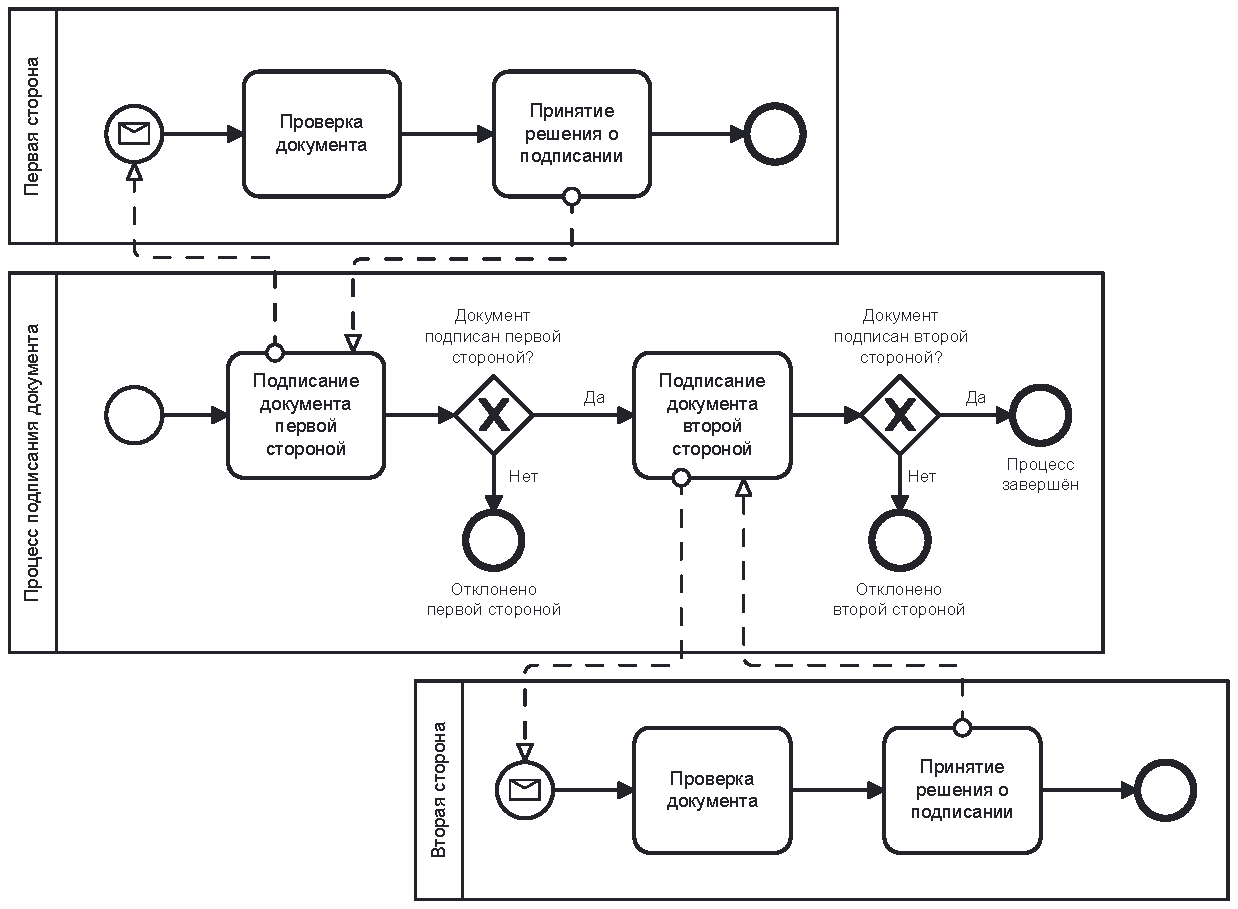
\includegraphics[width=0.9\textwidth]{inc/sign_flow_bpmn.pdf}
	\caption{Модель бизнесс-процесса подписания документа}
	\label{fig:sign-flow}	
\end{figure}

\clearpage

\section{Существующие решения}

В данном разделе будут рассмотрены наиболее популярные СЭД на российском рынке коммерческих и юридических услуг.

\subsection{Битрикс 24}

Комплексное предложение по оказанию цифровых услуг для бизнеса\cite{bitrix}. Система позволит создать архив документов, который будет автоматически пополняться новыми файлами (поступают с электронной почты или других источников). Ролевую модель можно настроить так, чтобы доступ к новым документам выделялся лишь определенным группам пользователей.

\subsection{СЭД от Сбербанка}

Система электронного документооборота от Сбербанка\cite{sber} позволит перевести всю офисную документацию в цифровой вид и получать к ней мгновенный доступ из любой точки мира. Система позволяет обмениваться документами с контрагентами и подписывать их с помощью электронной подписи. Статус документов на сервере обновляется в момент внесения изменений, что позволяет минимизирует смену состояния документа.

Также эта система ЭДО может самостоятельно собирать отчёты для государственных органов -- финансовой налоговой службы (ФНС) и Социального фонда России. Есть возможность работы с физлицами.

\subsection{1C: Документооборот}

1C: Документооборот -- Комплексный набор приложений, позволяющий настроить цифровую систему обмена документами внутри предприятия и с \\* контрагентами\cite{1c}. Система позволяет создавать хранилища документов, редактировать и шифровать их, выстраивать структуру и маршрут движения.

Файлы разрешено передавать через электронную почту, \texttt{FTP}-серверы или подключаемые веб-сервисы. Вместе с документами будут предоставляться сведения об электронной подписи. Реализована поддержка мобильного приложения, в котором можно полноценно работать со всеми функциями СЭД.

\subsection{СБИС}

Программа для управления бизнесом с продвинутым модулем электронного документооборота\cite{sbis}. Система позволяет создавать архив, настраивать обмен документов и работу с контрагентами.

\subsection{Alfresco Community Edition (CE)}

Бесплатное решение с открытым исходным кодом\cite{ace} (\texttt{Free Open} \\* \texttt{Source Software} -- \texttt{FOSS}). В данной СЭД отсутствует поддержка цифровой подписи из-за этого в ней невозможно проводить юридически значимые действия с контрагентами. Система позволяет создавать хранилища документов, редактировать и шифровать их, выстраивать структуру и маршрут движения.

\subsection{Вывод}

Сравним вышеперечисленные СЭД по следующим критериям:
\begin{enumerate}
	\item цена -- начальная цена предоставления услуг в выражении тысяч рублей (т.р.), бесплатном (Б) и условно-бесплатном (УБ);

	\item возможность СЭД организации хранения документов (архив);

	\item наличие СЭД в реестре ФНС;

	\item поддержка электронного документооборота (ЭДО);

	\item поддержка электронной подписи (ЭП) документов;

	\item поддержка предварительного согласования (С) документов;
	
	\item признак программного обеспечения с открытым исходным кодом (\texttt{FOSS}).
\end{enumerate}

 Все рассмотренных СЭД могут осуществлять ЭДО. Возможность использования электронной подписи и наличие в реестре ФНС есть только у проприетарных СЭД. Системы с открытым исходным кодом не подходят для обмена с контрагентами, но являются бесплатными и подойдут для работы внутри одного предприятия. Среди перечисленных СЭД возможность предварительного согласования есть только у СЭД от Сбербанка, так же она является условно бесплатной -- только для клиентов с расчётным счётом в данном банке, в отличие от других проприетарных СЭД, предоставляющих услуги на коммерческой основе. Результаты сравнения СЭД представлены в таблице \ref{tab:dbs}.

\begin{table}[h!]
	\begin{center}
		\caption{Сравнение СЭД}
		\label{tab:dbs}
		\begin{tabular}{|c|c|c|c|c|c|c|c|}
			\hline
			СЭД & Цена & Архив & ФНС & ЭДО & ЭП & С & FOSS\\
			\hline
			Битрикс 24 & от 7т.р. & + & + & + & + & - & - \\ \hline
			СЭД Сбербанка & УБ & + & + & + & + & + & -\\ \hline
			1С & от 43т.р. & +  & + & + & + & - & -\\ \hline
			СБИС & от 1.5т.р. & + & + & + & + & - & -\\ \hline
			Alfresco CE & Б & + & - & + & - & - & +\\ \hline
		\end{tabular}
	\end{center}
\end{table}

\clearpage

\section{Использование сетей Петри}

Сети Петри\cite{kotov-petri} представляют собой абстрактную формальную модель для описания и моделирования систем обработки информации. Моделирование в сетях Петри осуществляется на событийном уровне: определяются действия, происходящие в системе, состояние, предшествовавшее этим действиям, и какое состояние примет система после выполнения определённого действия. Выполнение событийной модели в сетях Петри описывает поведение системы. Для моделирования ЭДО рассмотрим раскрашенную сеть Петри\cite{kotov-petri} -- \texttt{Coloured Petri Net (CPN)}. 

\subsection{Раскрашенная сеть Петри}

Раскрашенная сеть Петри -- это кортеж, состоящий из восьми элементов:

\begin{equation}
	CPN = <P, I, T, G, A, E, Z, C>
\end{equation}

1. $P$ -- конечное множество позиций. С каждой позицией может
быть связана определённая маркировка, которая учитывает наличие
в данной позиции различных типов ресурсов. Маркировка позиции
$p \in P$ представляет собой мультимножество, например, следующего
вида: $m(p) = (1'r,2'b,1'g)$. Здесь $r, b, g$ -- переменные указанных цветовых типов, определяющие различные виды ресурсов, а цифры, стоящие перед апострофами, -- количество фишек соответствующего типа
в позиции $p \in P$.

2. $I(p)$ -- функция инициализации сети \texttt{CPN}.

3. $Т$ -- конечное множество переходов.

4. $G$ -- блокировочная функция, описывающая дополнительные условия, которые должны быть выполнены для срабатывания перехода $t \in T$.

5. $A$ -- конечное множество ветвей, связывающих между собой позиции и переходы.

6. $E(a)$ -- функция, задающая выражения на ветвях $a \in A$.

7. $Z$ -- конечное множество непустых типов, называемое цветами.

8. $C(p)$ -- цветовая функция, определяющая множество типов цветов, разрешённых для каждой позиции.

\subsection{Раскрашенная сеть Петри с временным механизмом}

Существует ряд задач моделирования, в которых необходимо учитывать не только последовательность событий, но и время их наступления, а также продолжительность. Для этой цели предусмотрено расширение возможностей раскрашенных сетей Петри\cite{kotov-petri} путем введения временного механизма -- \texttt{Timed CPN (tCPN)}:

\begin{equation}
	tCPN = <P, I, T, G, A, E, Z, C, \tau, \varDelta t>
\end{equation}

В модель системы вводятся часы, показывающие глобальное время $\tau$.

\subsection{Стохастические сети Петри}

Стохастические сети Петри -- модель количественного анализа дискретных динамических систем событий, основанная на концепции стохастических временных задержек\cite{spn}. Стохастические сети Петри объединяют многочисленные достоинства сетей Петри с возможностью оценки количественных характеристик более естественным образом, чем \texttt{tCPN}, поскольку многие реальные процессы лучше описываются вероятностными моделями.

\subsection{Использование сетей Петри для моделирования ЭДО}

Представим модель сети Петри для моделирования бизнес-процессов \\* ЭДО для документов с временными ограничениями (время выполнения обновления документа не должно превышать заданную продолжительность времени) и вероятностными переходами состояний в зависимости от содержания документа (отказ в согласовании, либо подтверждение). В качестве примера рассмотрим процесс формулировки и утверждения темы для выпускной квалификационной работы (ВКР). Модель бизнесс-процесса представлена на рисунке \ref{fig:vkr}.

\begin{figure}[h!btp]
	\centering
	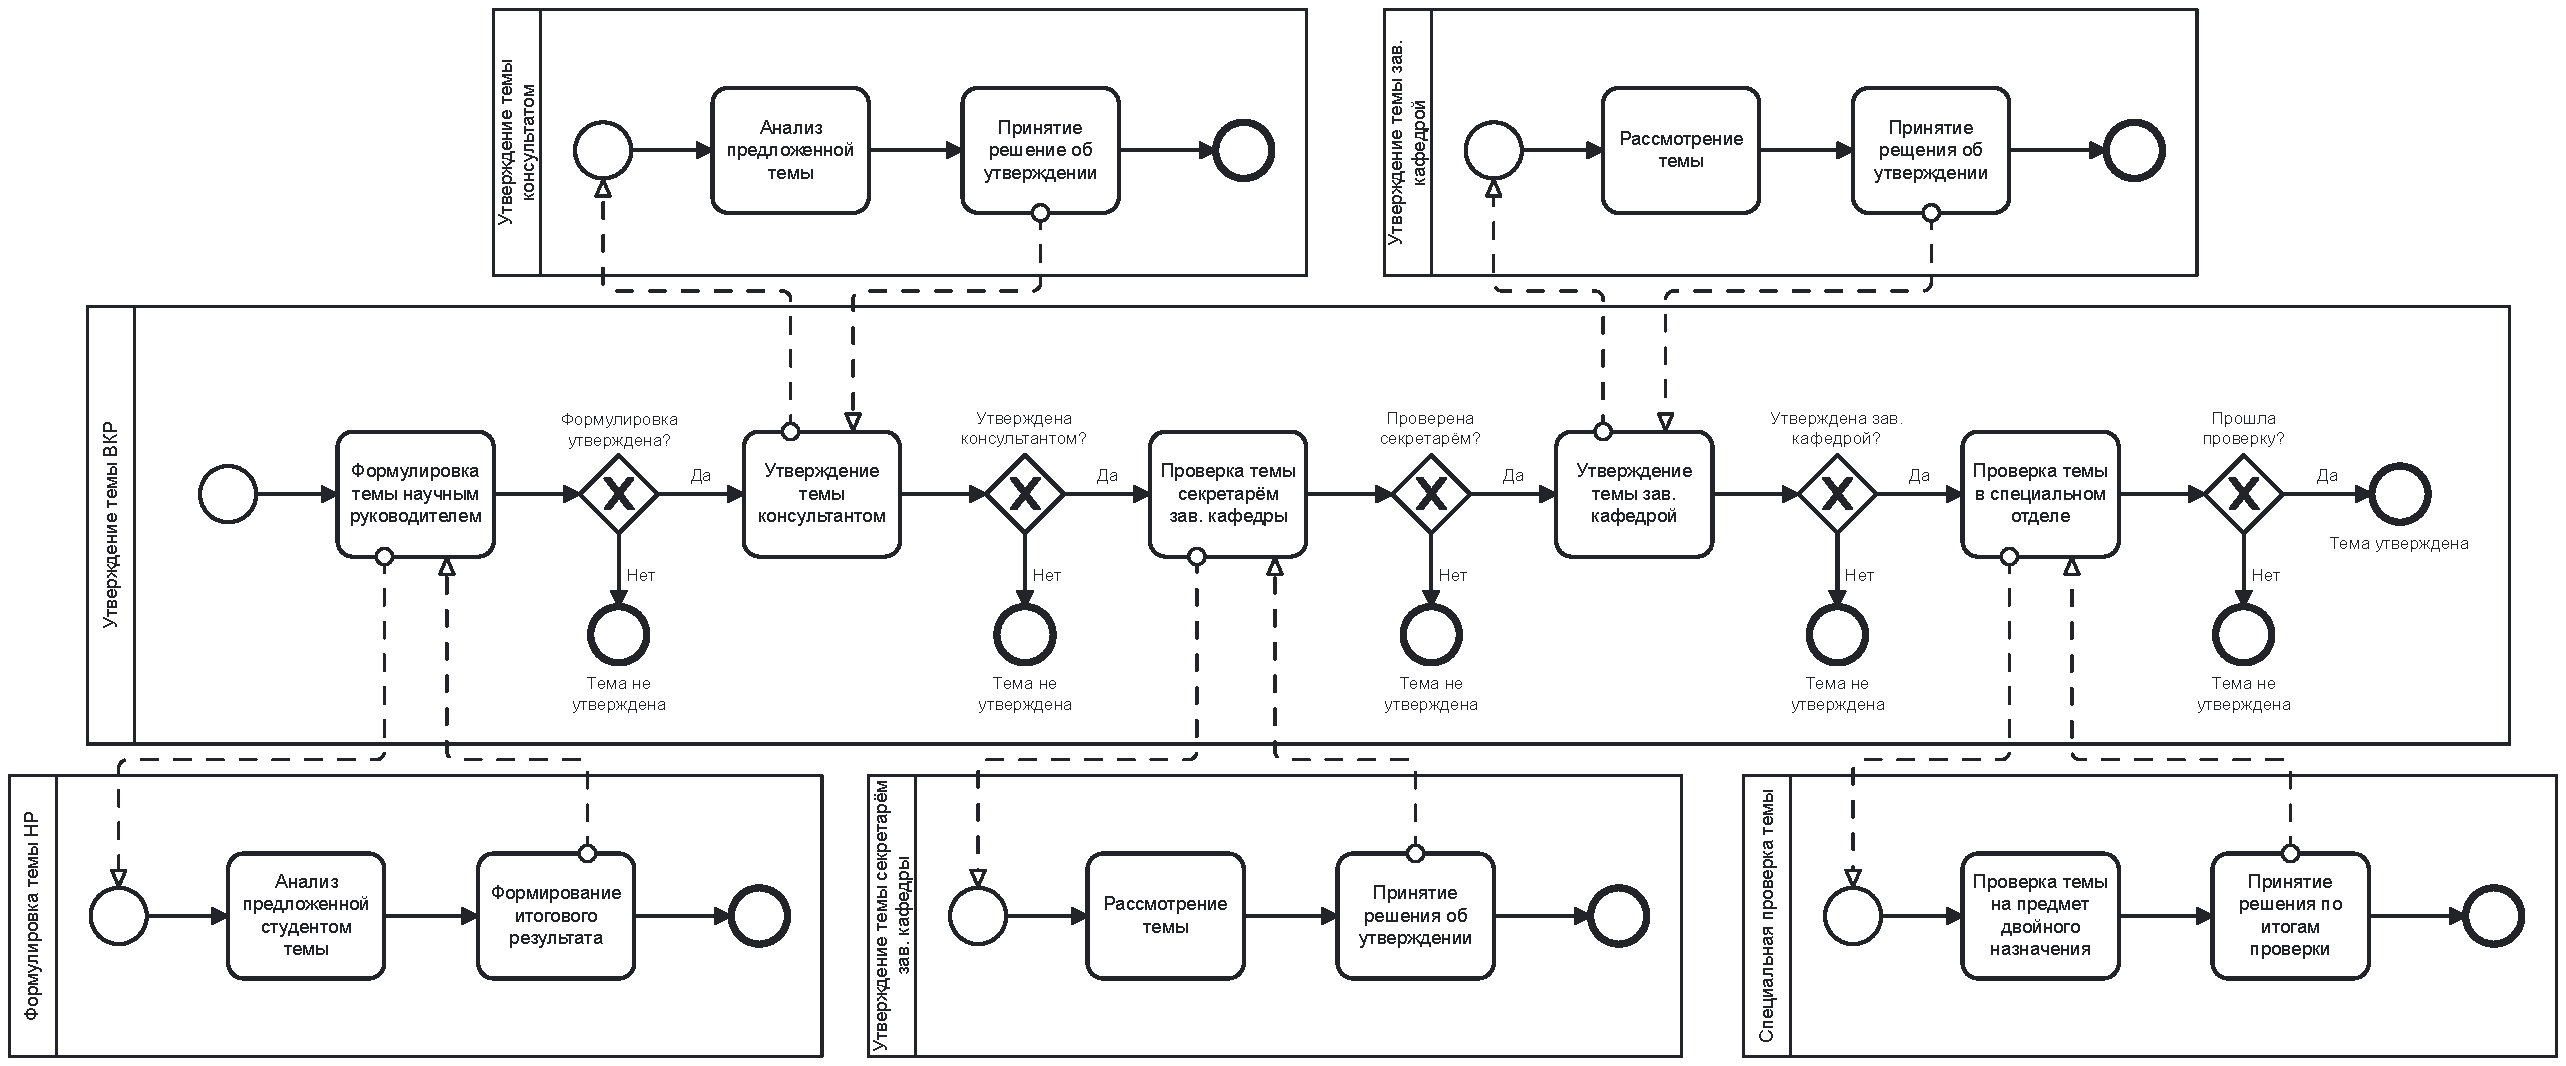
\includegraphics[width=\textwidth]{inc/vkr_bpmn.pdf}
	\caption{Модель бизнесс-процесса формулировки и утверждения темы ВКР}
	\label{fig:vkr}	
\end{figure}

\clearpage

Построим соответствующую процессу стохастическую модель сети Петри для дальнейшего моделирования процесса. В качестве инструмента для создания и моделирования сетей Петри используется программное обеспечение \texttt{Oris Tool}\cite{oris}. Итоговая модель сети Петри представлена на рисунке \ref{fig:tpn}.

\begin{figure}[h!btp]
	\centering
	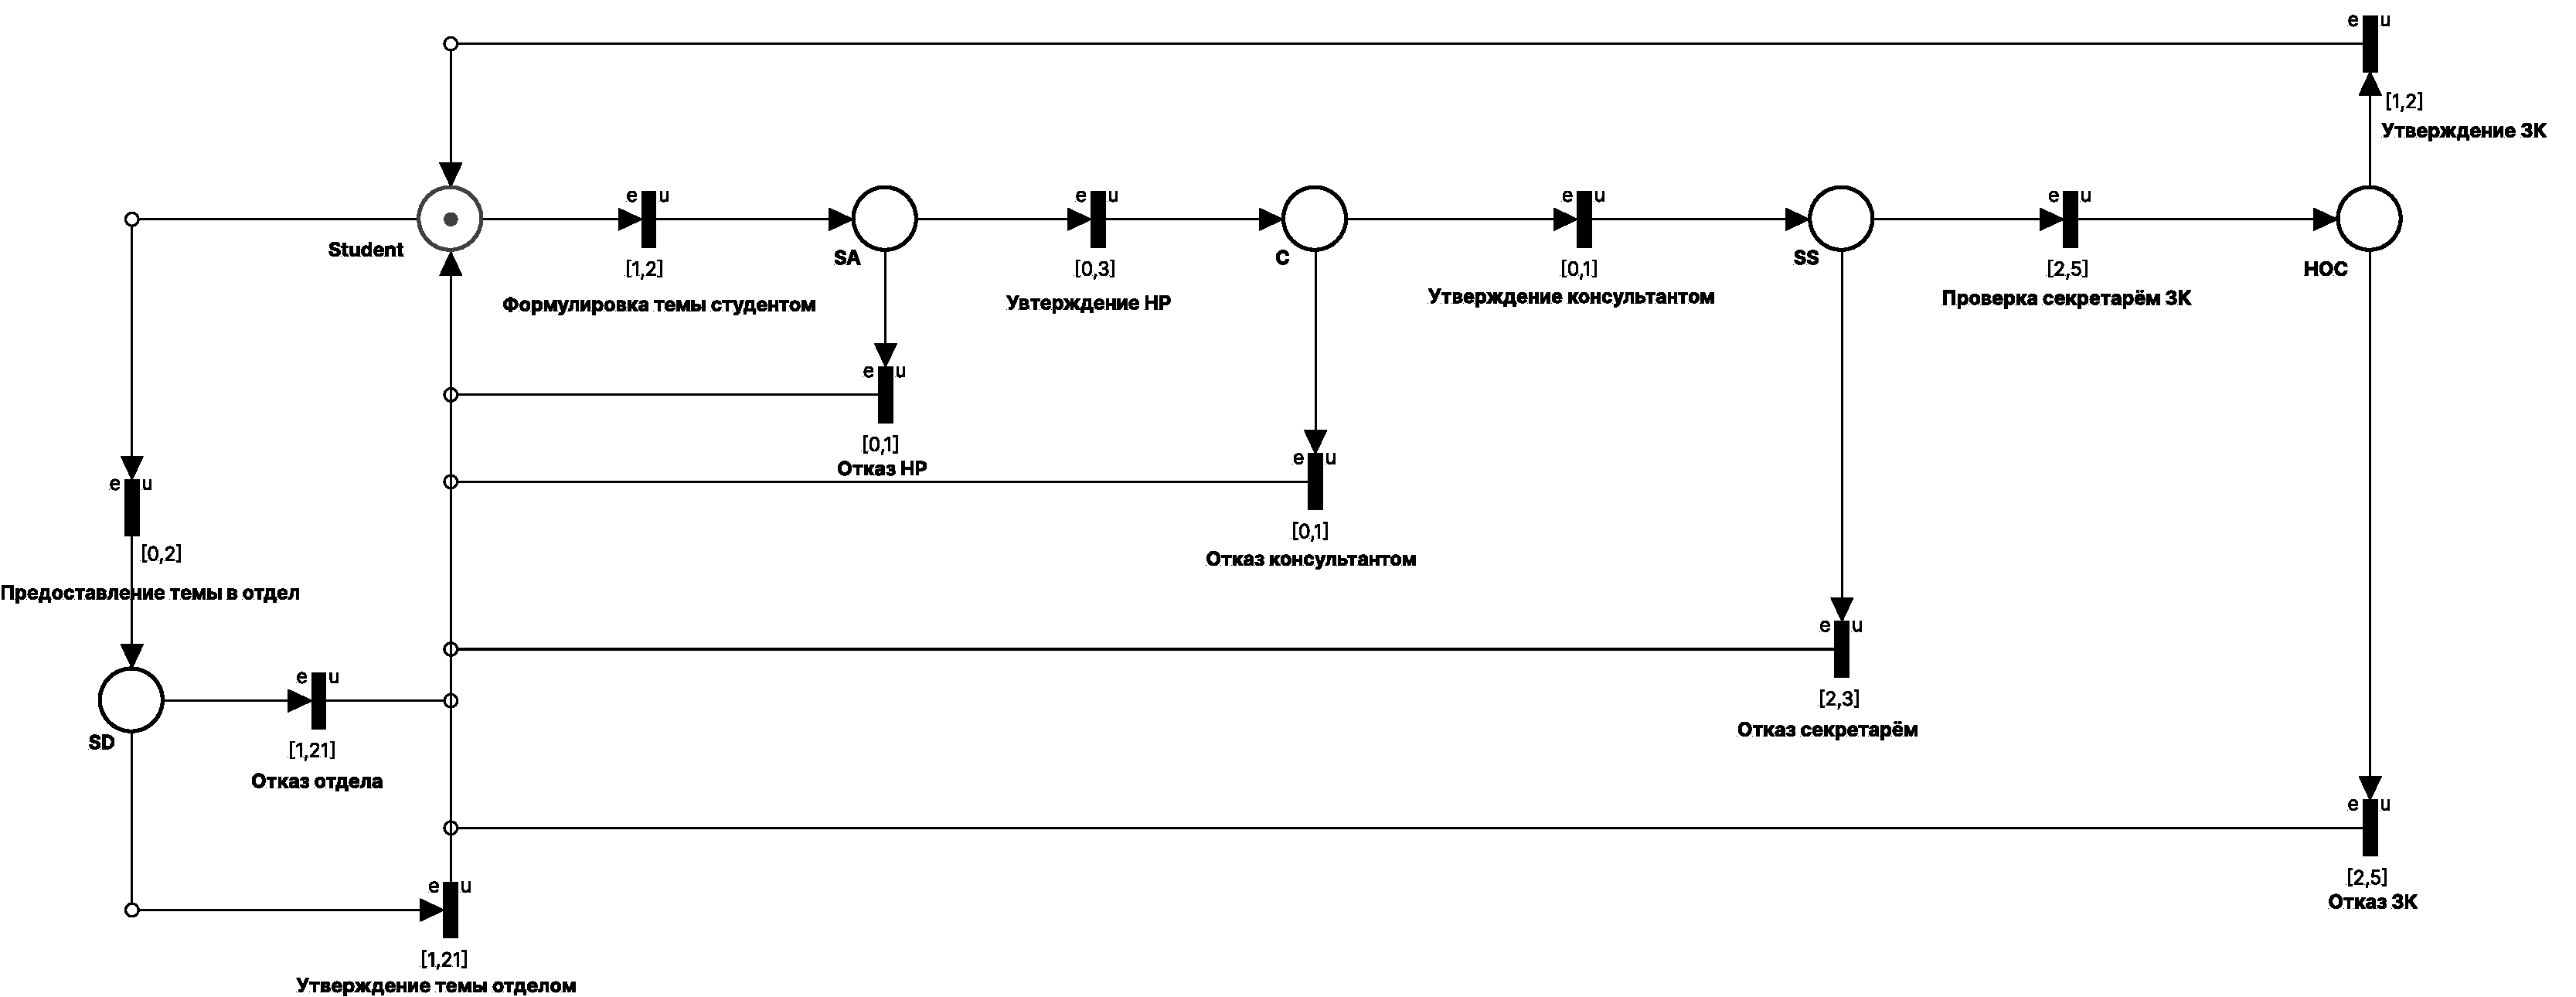
\includegraphics[width=\textwidth]{inc/timed.pdf}
	\caption{Модель сети Петри}
	\label{fig:tpn}	
\end{figure}

Прямой анализ переходных процессов\cite{forward-transient} на временном отрезке в 22 временных единицы показал сходимость модели к 20 временным единицам. Результат прямого анализа переходных процессов представлен на рисунке \ref{fig:ft}.

\begin{figure}[h!btp]
	\centering
	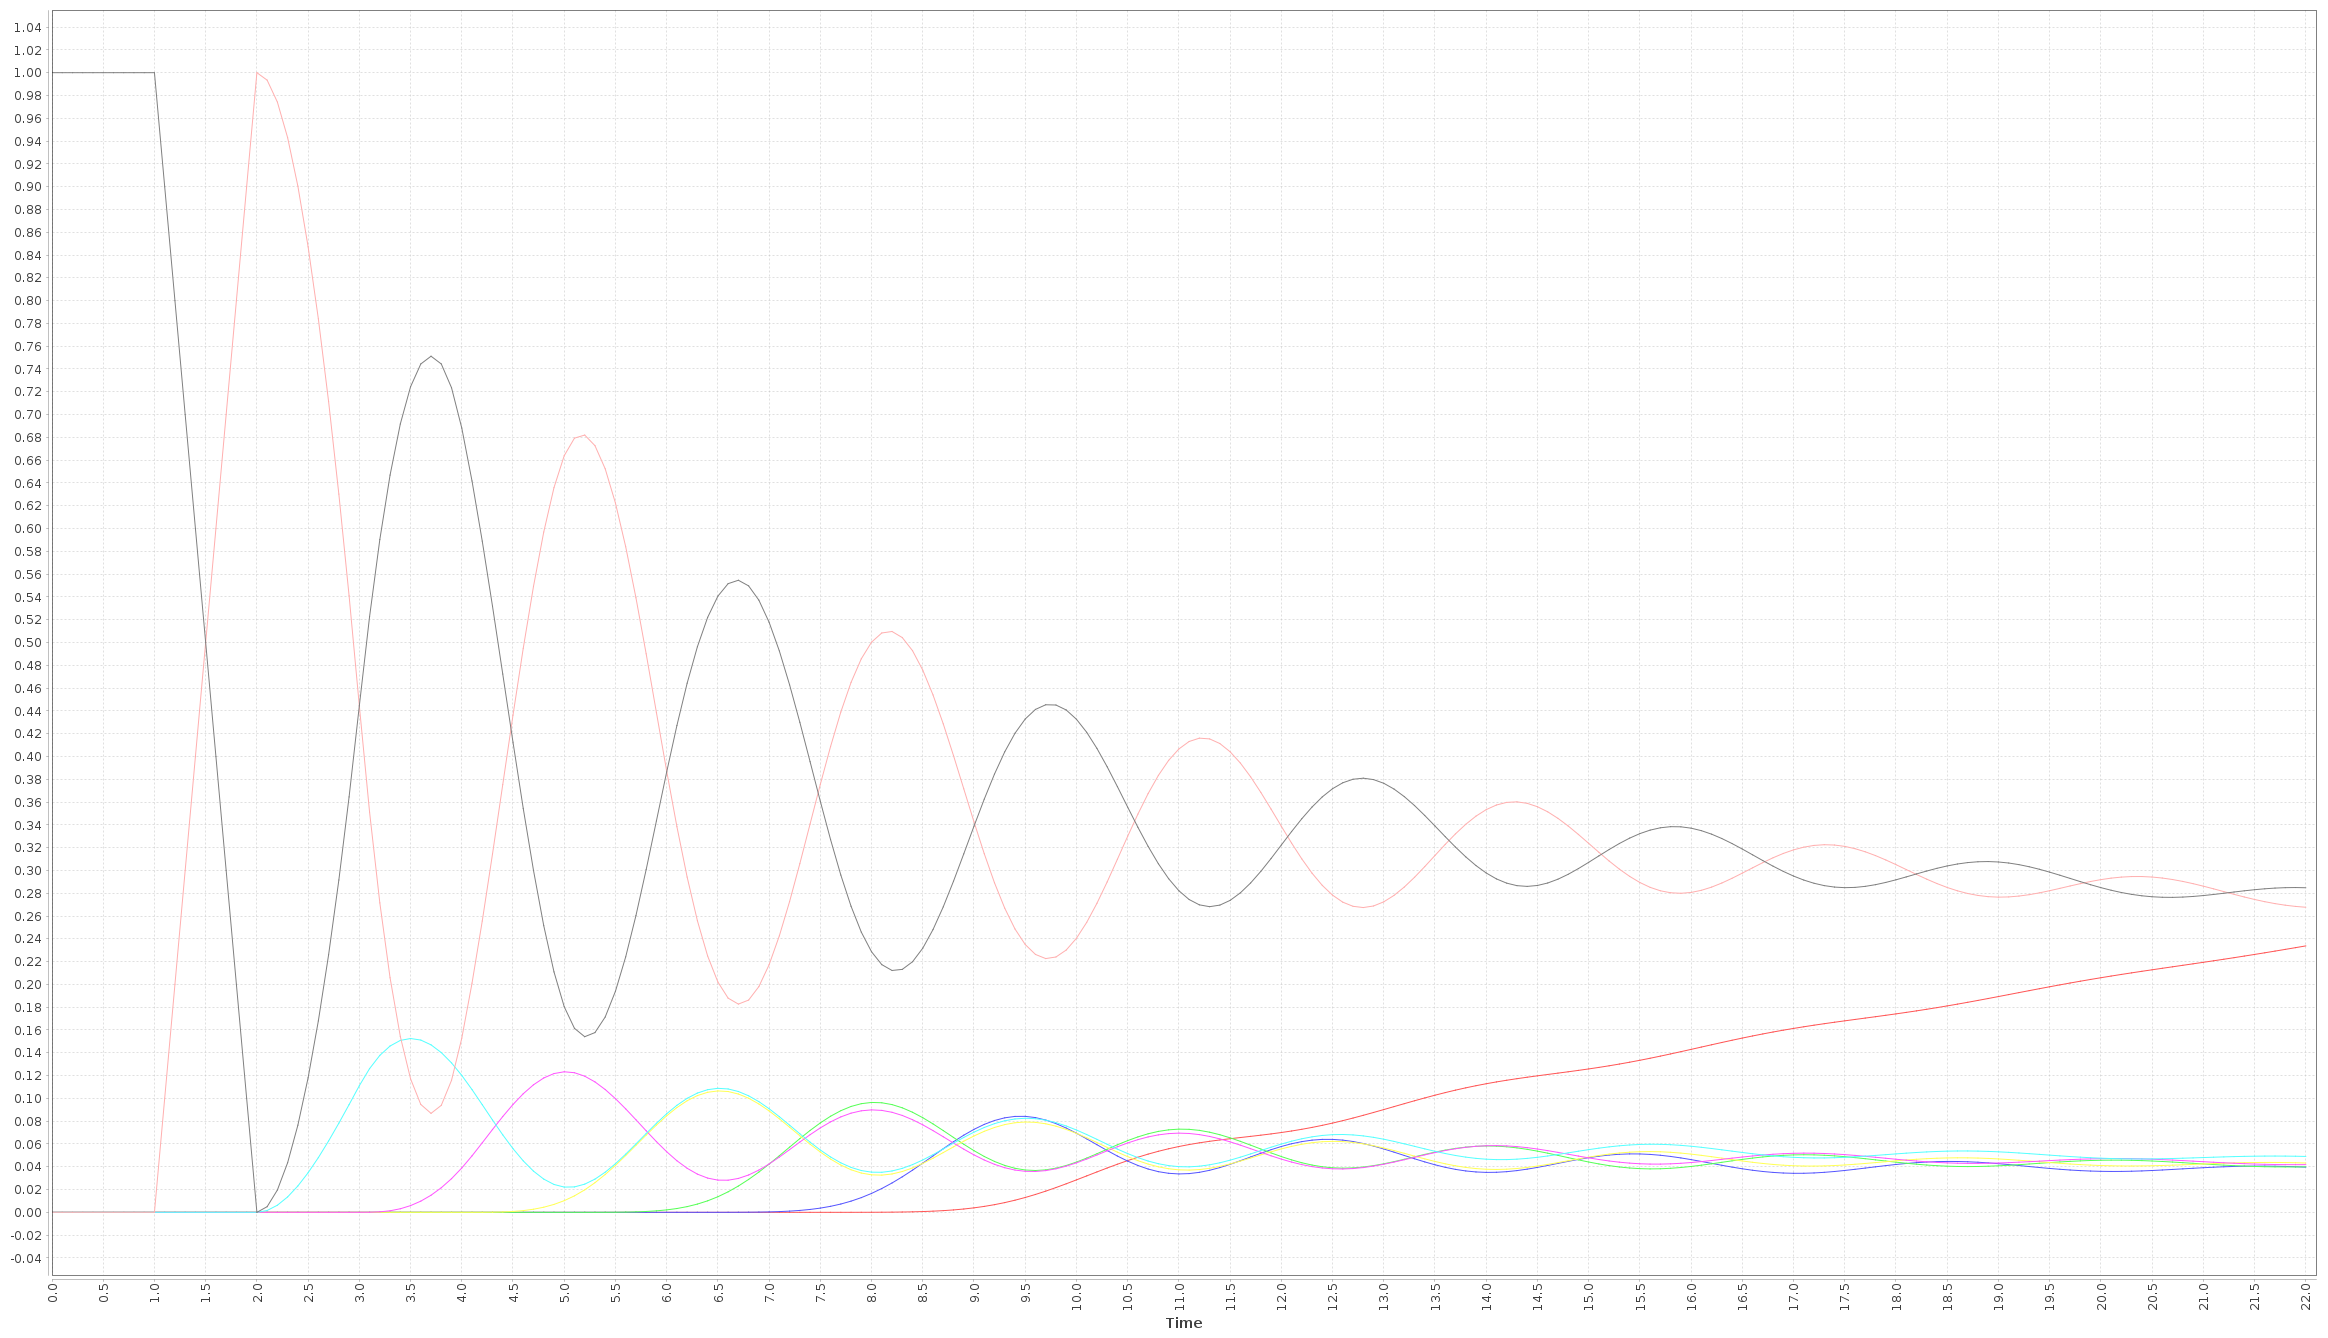
\includegraphics[width=0.9\textwidth]{inc/forward_transient.png}
	\caption{Результат прямого анализа переходных процессов}
	\label{fig:ft}
\end{figure}

Регенеративный анализ переходных процессов\cite{regenerative-transient} на временном отрезке в 34 временные единицы с использованием переменной, отвечающей за полное выполнение цикла модели -- \texttt{Reward variable}\cite{reward} подтвердил результаты прямого анализа. Результат регенеративного анализа переходных процессов представлен на рисунке \ref{fig:rt}.

\begin{figure}[h!btp]
	\centering
	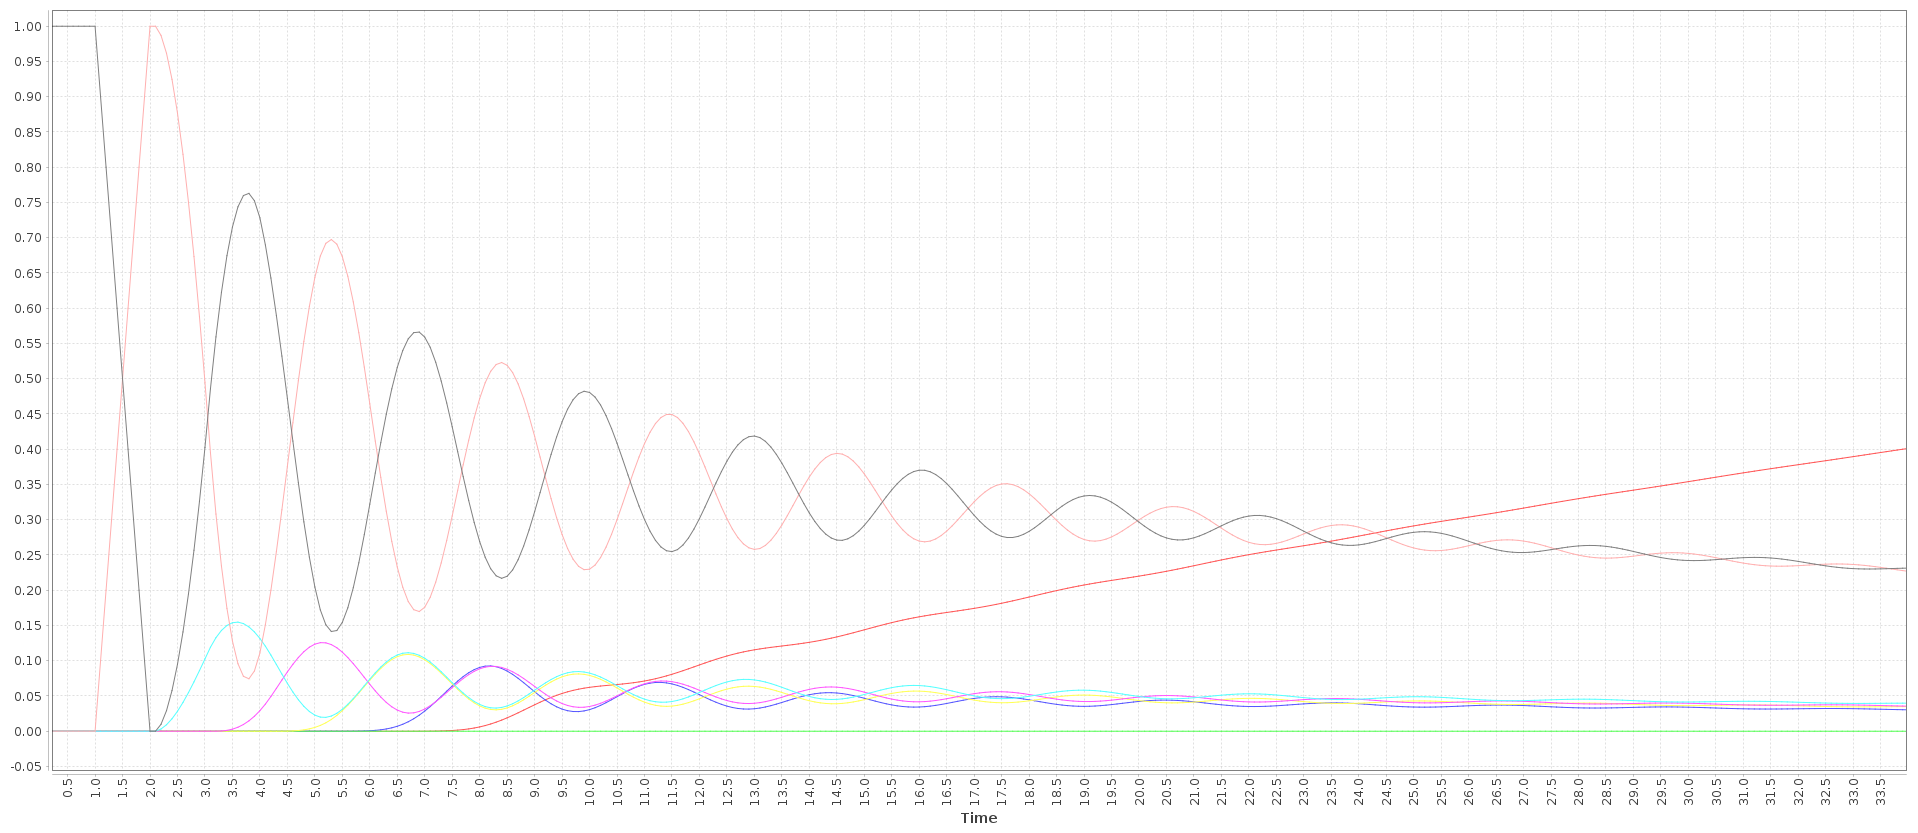
\includegraphics[width=0.9\textwidth]{inc/timed_reward.png}
	\caption{Результат регенеративного анализа переходных процессов}
	\label{fig:rt}
\end{figure}

Результаты заключительный регенеративный анализ для установления отношения вероятности достижения успешного исхода событий от времени представлены на рисунке \ref{fig:sp}.

\begin{figure}[h!btp]
	\centering
	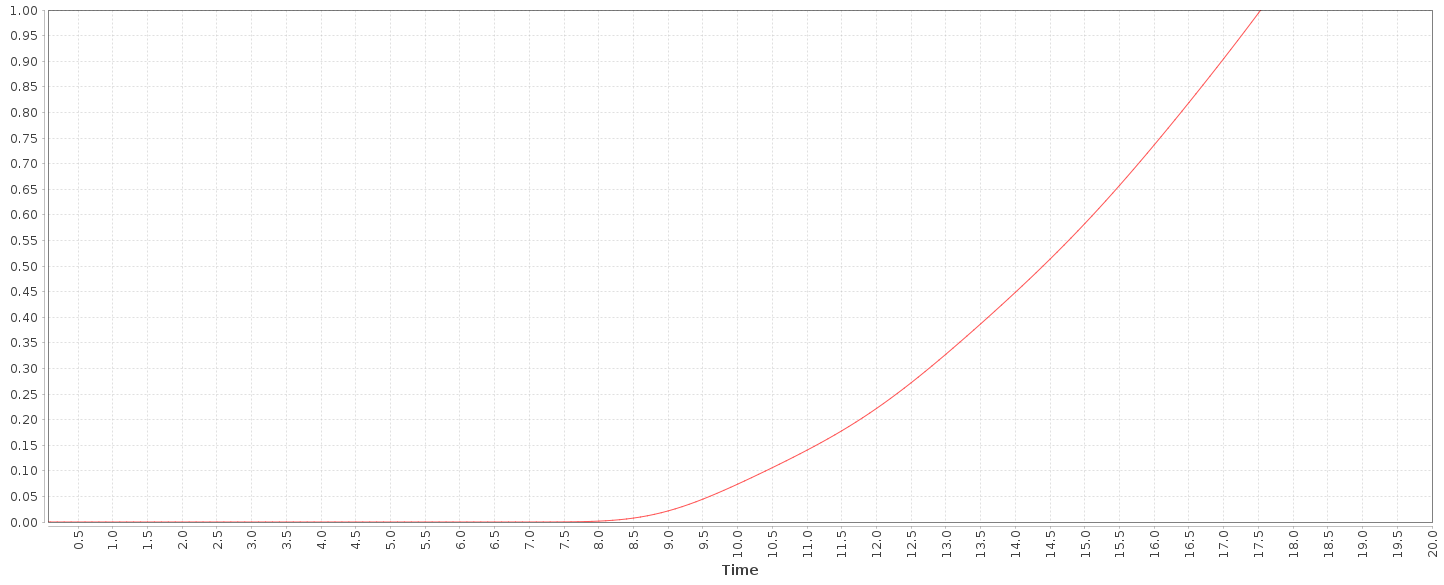
\includegraphics[width=0.9\textwidth]{inc/stud_prob.png}
	\caption{Результат регенеративного анализа переходных процессов}
	\label{fig:sp}
\end{figure}

Исходя из полученных данных прямого и обратного анализов максимальное время на выполнение процесса может занять до 18 временных единиц.

\clearpage

\specsection{ЗАКЛЮЧЕНИЕ}

В результате проведённого моделирования максимальное время выполнения процессов по утверждению темы для ВКР может составить до 18 временных единиц. На основе полученных данных руководством образовательного учреждения могут быть предприняты действия по улучшению текущих процессов путём возможного объединения промежуточных состояний, либо разбиением длительных состояний на более короткие последовательные.

Организовать выполнение данного процесса можно с помощью систем ЭДО, которые позволят сократить количество времени на переходах между возможными состояниями процесса.

\clearpage

\specsection{СПИСОК ИСПОЛЬЗОВАННЫХ ИСТОЧНИКОВ}
\addtolength{\oddsidemargin}{-0.25pt}
\begingroup
\renewcommand{\section}[2]{}
\bibliographystyle{utf8gost705u}
\bibliography{bibliography}   
\endgroup

\end{document}
